\header{8}
\chapter{Krachten op het schip}
\section{Inleiding}

Om optimaal gebruik van de wind te kunnen maken, is het van belang om de krachten en hun effecten op het schip te begrijpen. Door deze kennis juist toe te passen is het mogelijk om sneller en efficiënter te zeilen. De juiste kennis van krachten is ook handig voor een aantal zeilmanoeuvres. 

\section{Krachten en koppels}
\label{par:krachten_uitleg}
In dit hoofdstuk wordt gebruik gemaakt van twee eenvoudige natuurkundige principes: krachten en koppels. De theorie hierachter wordt daarom kort toegelicht.

\begin{figure}[H]
	\centering
	\begin{minipage}[t]{0.75\textwidth}
		\paragraph{Kracht}
		Wanneer een kracht op een voorwerp gezet wordt kunnen er twee dingen gebeuren: het voorwerp verplaatst of het voorwerp vervormt. In dit hoofdstuk wordt alleen gekeken naar het verplaatsende effect van een kracht. Een kracht is gedefinieerd door twee componenten: een richting en een grootte/sterkte. Een voorbeeld van een kracht op een boot is te zien in figuur  \ref{pic:kracht}. 
	\end{minipage}
	\hfill
	\begin{minipage}[t]{0.22\textwidth}
		\raisebox{-0.9\height}{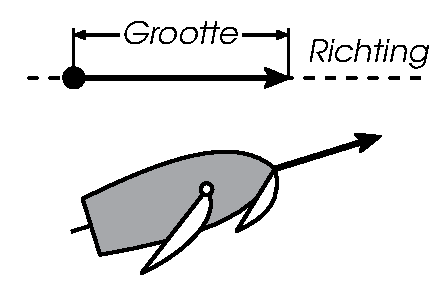
\includegraphics[width=\textwidth,]{Hoofdstukken/Krachten/pdf/kracht_op_vlet.pdf}}
		\RemoveLine
		\caption{}
		\label{pic:kracht}
	\end{minipage}
\end{figure} 

\paragraph{Krachten optellen en ontbinden}
Met krachten kan ook `gerekend' worden. Zo kunnen twee krachten die op hetzelfde voorwerp werken worden opgeteld. Een enkele kracht kan daarentegen worden opgedeeld in meerdere krachten met hetzelfde effect.

In figuur \ref{pic:kracht_som} zijn twee krachten te zien die op hetzelfde punt werken: blauw en rood. Door een parallellogram te maken van de krachten, is het mogelijk om de zwarte kracht te krijgen. Deze kracht heeft hetzelfde effect als de rode en blauwe kracht bij elkaar.

Het tegenovergestelde is ook mogelijk. Wanneer je een enkele kracht hebt, kun je deze splitsen in twee krachten met hetzelfde effect. In figuur \ref{pic:kracht_splits} is een enkele zwarte krachtpijl te zien. Deze wordt opgesplitst in de richting van rood en blauw.

Door een parallellogram om de zwarte kracht heen te tekenen, is het mogelijk lengte van de rode en blauwe kracht te bepalen. De zijdes vanuit de punt geven de krachten weer die hetzelfde effect hebben als de zwarte kracht.


\begin{figure}[H]
	\centering
	\begin{minipage}[b]{0.32\textwidth}
		\centering
		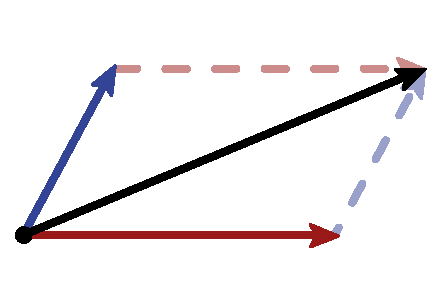
\includegraphics[width=0.85\textwidth]{Hoofdstukken/Krachten/pdf/kracht_optellen.pdf}
		\caption{Optellen}
		\label{pic:kracht_som}
	\end{minipage}
	\hfill
	\begin{minipage}[b]{0.32\textwidth}
		\centering
		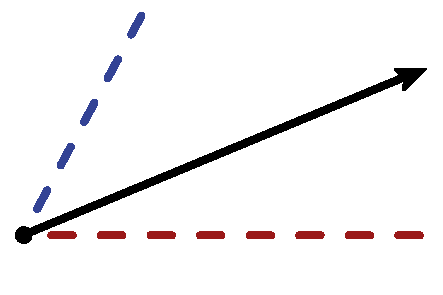
\includegraphics[width=0.85\textwidth]{Hoofdstukken/Krachten/pdf/kracht_richtingen.pdf}
		\caption{Enkele kracht}
		\label{pic:kracht_splits}
	\end{minipage}
	\hfill
	\begin{minipage}[b]{0.32\textwidth}
		\centering
		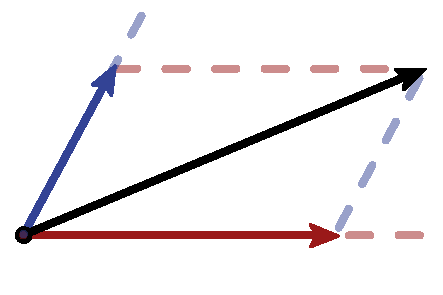
\includegraphics[width=0.85\textwidth]{Hoofdstukken/Krachten/pdf/kracht_splitsen.pdf}
		\caption{Gesplitste kracht}
		\label{pic:kracht_splits2}
	\end{minipage}
\end{figure}


\paragraph{Koppels en armen}
Een koppel is de natuurkundige beschrijving voor de kracht die een voorwerp doet draaien. In het voorbeeld in figuur \ref{pic:koppel} is een balk met een draaipunt te zien. Door een kracht op het einde van de balk te zetten zal er een draaiing ontstaan. Het effect van de kracht is een koppel om het draaipunt.

\begin{figure}[H]
	\centering
	\begin{minipage}[b]{0.49\textwidth}
		\centering
		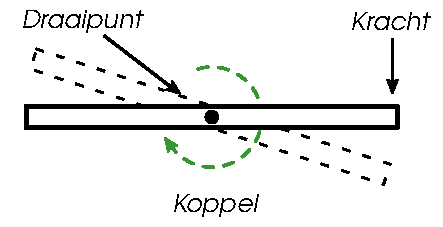
\includegraphics[width=0.75\textwidth]{Hoofdstukken/Krachten/pdf/kracht_koppel.pdf}
		\caption{Koppel}
		\label{pic:koppel}
	\end{minipage}
	\hfill
	\begin{minipage}[b]{0.49\textwidth}
		\centering
		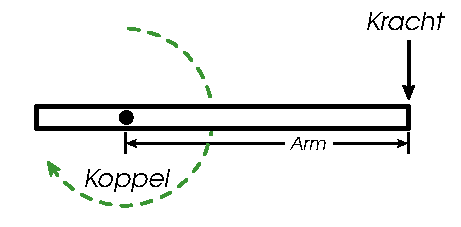
\includegraphics[width=0.75\textwidth]{Hoofdstukken/Krachten/pdf/kracht_arm.pdf}
		\caption{Arm}
		\label{pic:arm}
	\end{minipage}
\end{figure}
De afstand tussen de kracht en het draaipunt wordt ook wel de arm genoemd. Door de arm te vergroten is het mogelijk om met dezelfde kracht, een sterkere koppel te maken. Dit is weergegeven in figuur \ref{pic:arm}. De arm versterkt hier de kracht die op de balk geplaatst wordt.

\section{Voortstuwing van de boot}
Nu de basiskennis over de krachten is verworven, kan er verder gekeken worden naar hoe een boot voortgestuwd wordt. Dit wordt in drie stappen toegelicht: voortstuwende werking van de zeilen, driftbeperkende middelen en tot slot voortstuwing.

\subsection*{Voortstuwende werking van de zeilen}
De voortstuwende werking van de zeilen heeft alles te maken met de stroming van de wind langs de zeilen. In figuur \ref{pic:stroming} is een versimpeling van deze stroming te zien langs de fok en het grootzeil. 

Door de bolle vorm van de zeilen moet de wind aan de bolle zijde een langere weg afleggen dan aan de holle zijde. Hierdoor zal de wind aan de bolle zijde sneller stromen dan de holle zijde. Sneller stromende lucht heeft een lagedruk. Hierdoor ontstaat een drukverschil zoals te zien is in figuur \ref{pic:druk}.

\begin{figure}[H]
	\centering
	\begin{minipage}[b]{0.32\textwidth}
		\centering
		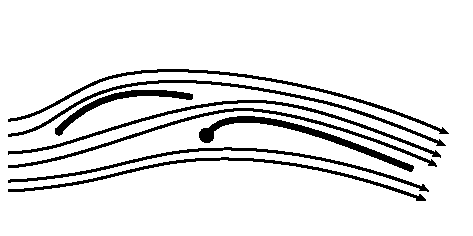
\includegraphics[width=0.95\textwidth]{Hoofdstukken/Krachten/pdf/voortstuwing_zeil_stroming.pdf}
		\caption{Stroming}
		\label{pic:stroming}
	\end{minipage}
	\hfill
	\begin{minipage}[b]{0.32\textwidth}
		\centering
		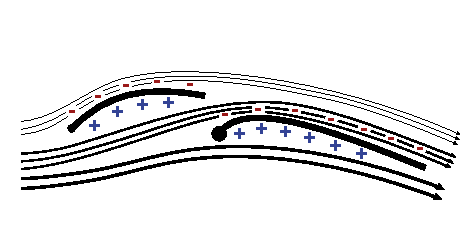
\includegraphics[width=0.95\textwidth]{Hoofdstukken/Krachten/pdf/voortstuwing_zeil_druk.pdf}
		\caption{Druk}
		\label{pic:druk}
	\end{minipage}
	\hfill
	\begin{minipage}[b]{0.32\textwidth}
		\centering
		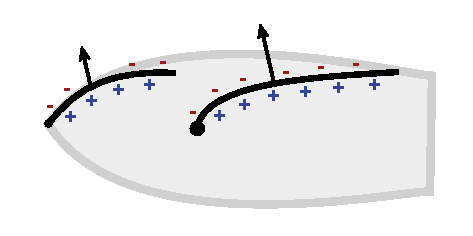
\includegraphics[width=0.95\textwidth]{Hoofdstukken/Krachten/pdf/voortstuwing_zeil_krachten_los.pdf}
		\caption{Voortstuwing}
		\label{pic:stuwing}
	\end{minipage}
\end{figure}

Omdat de lucht van het hoge naar het lage druk gebied toe wil, ontstaat er een kracht op beide zeilen. Wanneer je per zeil alle krachten opsomt, krijg je de krachten te zien in figuur \ref{pic:stuwing}.

\begin{figure}[H]
	\centering
	\begin{minipage}[t]{0.63\textwidth}
		\vspace*{0.2cm}
		Om makkelijk met deze krachten te werken nemen we de kracht van zowel de fok als het grootzeil samen. Dit levert de kracht in figuur \ref{pic:zeilpunt} op en heet de zeilkracht. Het punt waaruit de zeilkracht werkt noemen we het zeilpunt. 
	\end{minipage}
	\hfill
	\begin{minipage}[t]{0.32\textwidth}
		\raisebox{-0.9\height}{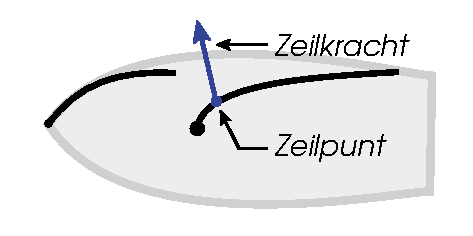
\includegraphics[width=0.95\textwidth]{Hoofdstukken/Krachten/pdf/voortstuwing_zeil_zeilkracht.pdf}}
		\RemoveLine
		\caption{Zeilpunt}
		\label{pic:zeilpunt}
	\end{minipage}
\end{figure} 

\subsection{Driftbeperkende middelen}
Om te voorkomen dat de zeilkracht de boot enkel verlijerd of drift, heeft deze driftbeperkende middelen. Deze middelen maken het lastiger voor de boot om zijwaarts over het water te bewegen doordat deze dwars op de boot staan. Een lelievlet beschikt over vier driftbeperkende middelen: het onderwaterschip, het zwaard, de skeg en het roer. In figuur \ref{pic:drift_beperking} zijn deze onderdelen afgebeeld.

\begin{figure}[H]
	\centering
	\begin{minipage}[b]{0.48\textwidth}
		\centering
		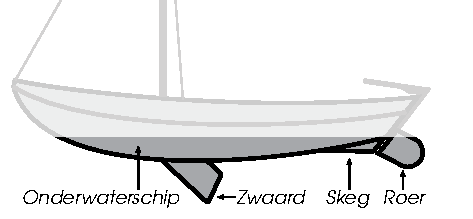
\includegraphics[width=0.90\textwidth]{Hoofdstukken/Krachten/pdf/lateraal_driftbeperking.pdf}
		\caption{Driftbeperking}
		\label{pic:drift_beperking}
	\end{minipage}
	\hfill
	\begin{minipage}[b]{0.48\textwidth}
		\centering
		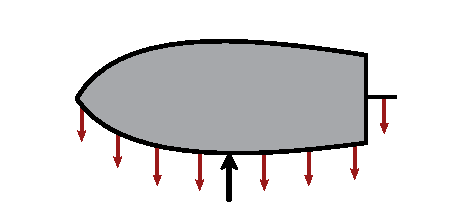
\includegraphics[width=0.90\textwidth]{Hoofdstukken/Krachten/pdf/lateraal_boven.pdf}
		\caption{Zijwaartse kracht}
		\label{pic:zijwaarts}
	\end{minipage}
\end{figure}
Om de driftbeperking en de krachten die hierbij komen kijken beter te begrijpen, kijken we naar de volgende situatie: een boot wordt door een externe kracht zijwaarts over het water geduwd. Dit is uitgebeeld in figuur \ref{pic:zijwaarts}. De zwarte pijl stelt het duwen van de boot voor. 

Wanneer de boot zijwaarts verplaatst wordt, zullen de driftbeperkende middelen dit tegengaan omdat deze het water om zich heen moeten verplaatsen. In figuur \ref{pic:zijwaarts} is de weerstand die deze middelen geven met de rode pijlen uitgebeeld. Figuur \ref{pic:zijwaarts_totaal} toont een zijaanzicht van deze situatie.

\begin{figure}[H]
	\centering
	\begin{minipage}[b]{0.48\textwidth}
		\centering
		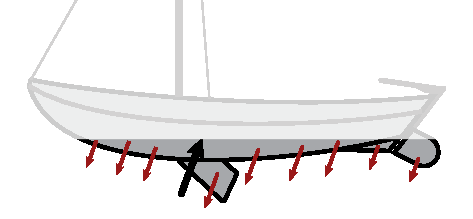
\includegraphics[width=0.90\textwidth]{Hoofdstukken/Krachten/pdf/lateraal_zij.pdf}
		\caption{Zijwaartse kracht zijaanzicht}
		\label{pic:zijwaarts_totaal}
	\end{minipage}
	\hfill
	\begin{minipage}[b]{0.48\textwidth}
		\centering
		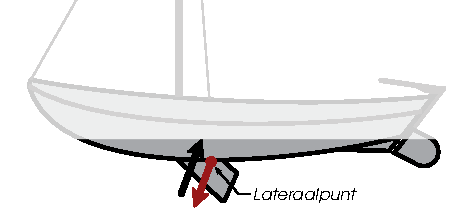
\includegraphics[width=0.90\textwidth]{Hoofdstukken/Krachten/pdf/lateraal_punt.pdf}
		\caption{Lateraalpunt}
		\label{pic:lateraal}
	\end{minipage}
\end{figure}

Wanneer we al deze krachten sommeren krijgen we een totaal kracht (rood) die is afgebeeld in figuur \ref{pic:lateraal}. Deze kracht werkt vanuit een punt dat ook wel het lateraalpunt genoemd wordt. Het lateraalpunt is formeel gedefinieerd als: ``\textit{Het punt waar alle laterale (zijwaartse) krachten van het schip op werken}''. Het lateraalpunt is tevens het draaipunt van het schip.

Door middel van het lateraalpunt kan makkelijk gerekend worden met de driftbeperkende kracht van het schip. Dit zal van pas komen in het begrijpen van de voortstuwing van de boot.

\newpage
\subsection{Voortstuwing}
Met de kennis die is opgedaan over zowel de zeil- als driftbeperkende kracht is het mogelijk om te kijken naar hoe de boot vooruit bewogen wordt. In figuur \ref{pic:krachten_los} is een boot te zien samen met een zeilkracht (blauw) en een driftbeperkende kracht (rood). Deze krachten zijn getekend vanuit het zeilpunt en het lateraalpunt.

\begin{figure}[H]
	\centering
	\begin{minipage}[b]{0.48\textwidth}
		\centering
		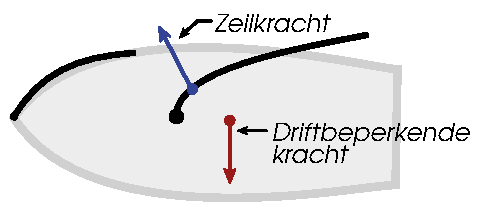
\includegraphics[width=0.90\textwidth]{Hoofdstukken/Krachten/pdf/voortstuwing_krachten.pdf}
		\caption{Zeil en drifbeperkende kracht}
		\label{pic:krachten_los}
	\end{minipage}
	\hfill
	\begin{minipage}[b]{0.48\textwidth}
		\centering
		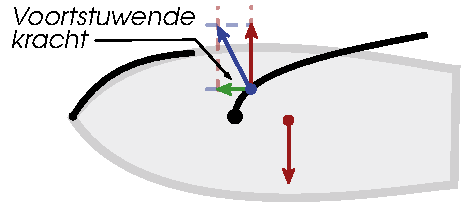
\includegraphics[width=0.90\textwidth]{Hoofdstukken/Krachten/pdf/voortstuwing_totaal.pdf}
		\caption{Voortstuwende kracht}
		\label{pic:voorwaardse_kracht}
	\end{minipage}
\end{figure}

In figuur \ref{pic:voorwaardse_kracht} wordt de zeilkracht gesplitst in twee krachten met hetzelfde effect: de voorwaartse kracht (groen) en de verlijerende kracht (rood). De verlijerende kracht wordt echter opgeheven door de driftbeperkende kracht. Hierdoor blijft alleen de voortstuwende kracht nog over. Deze samenwerking van de krachten geeft een zeilboot zijn voortstuwing.

\section{Correcte zeilstand}
Door de zeilen in een correcte stand te zetten is het mogelijk de voortstuwende werking hiervan te optimaliseren. Dit heet ook wel het trimmen van de zeilen. Een correct getrimd zeil is weergegeven in figuur \ref{pic:zeil_goed}. In dit figuur is te zien dat de stroming van de wind de zeilen strak volgt. Deze stroming creëert zo het grootste drukverschil en hiermee de meeste voortstuwing. 

Wanneer het zeil echter te strak staat, ontstaat de situatie in figuur \ref{pic:zeil_strak}. De windstroming laat halverwege het grootzeil `los'. Dit zorgt voor turbulentie aan het achterlijk van het zeil waardoor deze gaat klapperen. De verstoring in de stroming en de turbulentie verlagen het drukverschil tussen beide zijde van het zeil. Dit zorgt vervolgens voor een lagere voortstuwing.

\begin{figure}[H]
  \centering
  \begin{minipage}[b]{0.32\textwidth}
  \centering
    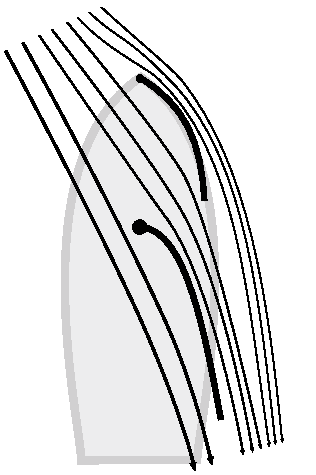
\includegraphics[height=5cm]{Hoofdstukken/Krachten/pdf/trimmen_goed.pdf}
    \caption{Zeil goed}
    \label{pic:zeil_goed}
  \end{minipage}
  \hfill
  \begin{minipage}[b]{0.32\textwidth}
    \centering
    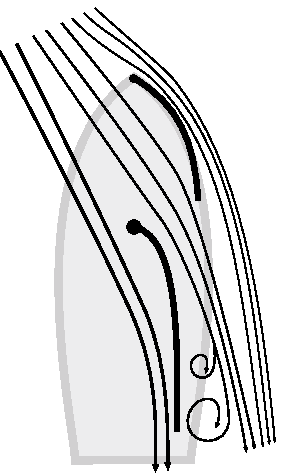
\includegraphics[height=5cm]{Hoofdstukken/Krachten/pdf/trimmen_strak.pdf}
    \caption{Zeil te strak}
    \label{pic:zeil_strak}
    \end{minipage}
  \hfill
  \begin{minipage}[b]{0.32\textwidth}
    \centering
    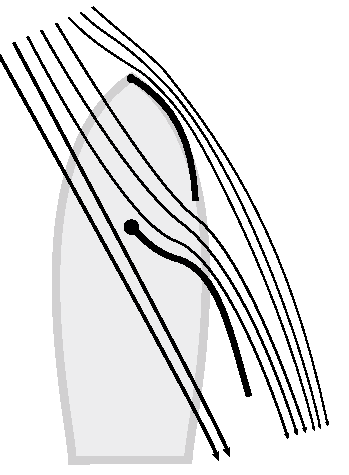
\includegraphics[height=5cm]{Hoofdstukken/Krachten/pdf/trimmen_los.pdf}
    \caption{Zeil te los}
    \label{pic:zeil_los}
  \end{minipage}
\end{figure}

In figuur \ref{pic:zeil_los} is een te los zeil te zien. De windstromen aan de hoge kant van het zeil volgen het zeil niet strak en aan de lage zijde wordt de stroming omgeleid door het zeil. Deze verstoringen in de stroming zorgen voor een lager drukverschil en minder voortstuwing. 

Een goede manier om je zeil te trimmen is om hem net zo lang te laten vieren totdat er een kleine tegenbolling in het voorlijk te zien valt. Daarna trek je het zeil weer een klein beetje aan tot deze weg valt. Op deze manier benut je de wind maximaal. Door dit regelmatig te doen weet je zeker dat je optimaal zeilt. 

\section{Effecten van de fok en het grootzeil}
Het grootzeil en de fok hebben allebei een ander effect op de koers van boot. Het verschil in dit gedrag is te verklaren door hun positie ten opzichte van het lateraalpunt. Omdat het grootzeil (en het bijbehorende zeilpunt) zich achter het lateraalpunt bevindt, creëert het grootzeil een oploevend koppel. Dit effect is weergegeven in figuur \ref{pic:effect_grootzeil}.

Het omgekeerde is waar voor de fok. Doordat deze zich voor het lateraalpunt bevindt, ontstaat er een afvallend koppel. Figuur \ref{pic:effect_fok} toont deze situatie. 

\begin{figure}[ht]
	\centering
	\begin{minipage}[b]{0.49\textwidth}
		\centering
		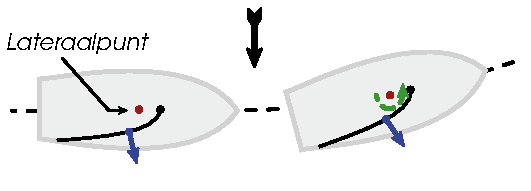
\includegraphics[width=\textwidth]{Hoofdstukken/Krachten/pdf/effect_grootzeil.pdf}
		\caption{Effect van het grootzeil}
		\label{pic:effect_grootzeil}
	\end{minipage}
	\hfill
	\begin{minipage}[b]{0.49\textwidth}
		\centering
		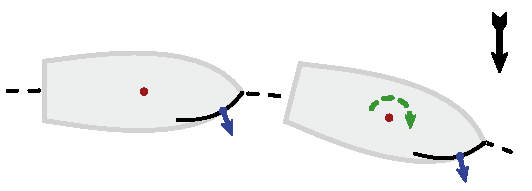
\includegraphics[width=\textwidth]{Hoofdstukken/Krachten/pdf/effect_fok.pdf}
		\caption{Effect van de fok}
		\label{pic:effect_fok}
	\end{minipage}
\end{figure}

Door gebruikt te maken van de sturende werking van de zeilen is het mogelijk de boot van koers te veranderen met minder gebruik van het roer. Hiermee wordt het oploeven en afvallen efficiënter.

\section{Effect van de helling}
Een lelievlet is van nature loefgierig. Dit houdt in dat de boot met een normale zeilstand maar zonder roer, de wind in draait. Door de helling van de boot te veranderen is het mogelijk om de loef- en lijgierigheid hiervan aan te passen.

De loefgierigheid van de boot komt voort uit de positie van het zeilpunt ten opzichte van het lateraalpunt. Dit is duidelijk te zien in het achteraanzicht van een boot in figuur \ref{pic:helling_vlak_achter}. Tussen het zeilpunt en het lateraalpunt bevindt zich een arm. Omdat het lateraalpunt tevens het draaipunt van de boot is, zorgt deze arm voor een koppel om het lateraalpunt waardoor de boot wil oploeven. Dit koppel is weergegeven in figuur \ref{pic:helling_valk_boven}. De arm tussen het zeilpunt en het lateraalpunt geeft de boot dus zijn loefgierheid.

\begin{figure}[H]
	\centering
	\begin{minipage}[b]{0.48\textwidth}
		\centering
		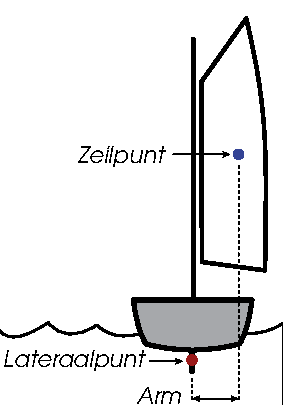
\includegraphics[height=5cm]{Hoofdstukken/Krachten/pdf/helling_vlak_achter.pdf}
		\caption{Zeilpunt en lateraalpunt}
		\label{pic:helling_vlak_achter}
	\end{minipage}
	\hfill
	\begin{minipage}[b]{0.48\textwidth}
		\centering
		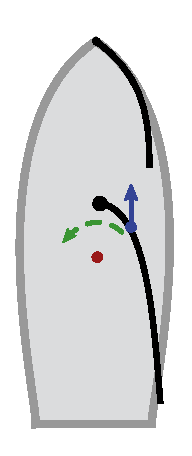
\includegraphics[height=5cm]{Hoofdstukken/Krachten/pdf/helling_vlak_boven.pdf}
		\caption{Oploevend koppel}
		\label{pic:helling_valk_boven}
	\end{minipage}
\end{figure}


De helling van de boot heeft een invloed op de lengte van deze arm. Door de boot meer naar de lijkant te hellen wordt de arm vergroot. Dit zorgt vervolgens voor een groter oploevend koppel. Figuur \ref{pic:helling_oploeven} laat deze vergrootte arm zien. 

\begin{figure}[H]
	\centering
	\begin{minipage}[b]{0.48\textwidth}
		\centering
		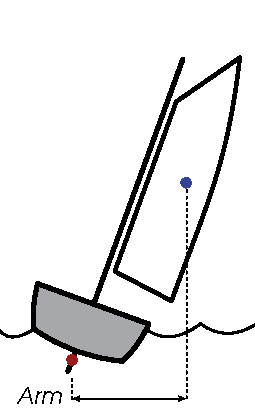
\includegraphics[height=5cm]{Hoofdstukken/Krachten/pdf/helling_lij_achter.pdf}
		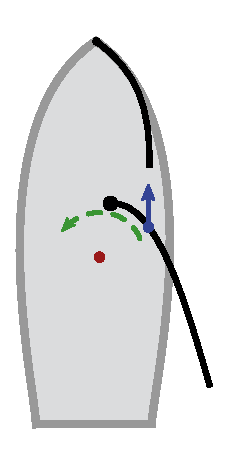
\includegraphics[height=5cm]{Hoofdstukken/Krachten/pdf/helling_lij_boven.pdf}
		\caption{Helling naar lij}
		\label{pic:helling_oploeven}
	\end{minipage}
	\hfill
	\begin{minipage}[b]{0.48\textwidth}
		\centering
		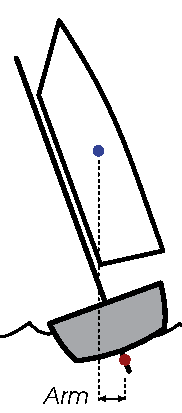
\includegraphics[height=5cm]{Hoofdstukken/Krachten/pdf/helling_loef_achter.pdf}
		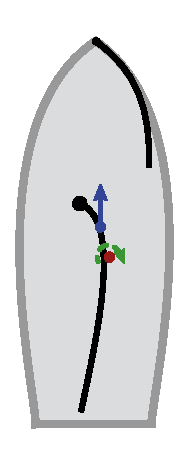
\includegraphics[height=5cm]{Hoofdstukken/Krachten/pdf/helling_loef_boven.pdf}
		\caption{Helling naar loef}
		\label{pic:helling_afvallen}
	\end{minipage}
\end{figure}

Het tegenovergestelde is ook mogelijk: door de boot te hellen naar de loefzijde, wordt de arm verkleind of zelfs omgedraaid. Dit zorgt ervoor dat de boot lijgierig wordt. Dit wordt weergegeven in figuur \ref{pic:helling_afvallen}.


Door correct gebruik te maken van de helling van het schip, is het mogelijk sneller en efficiënter af te vallen en op te loeven. Tijdens complexe manoeuvres biedt dit extra controle over de boot.  

\section{Stabiliteit}
De zeilkracht die de boot voortstuwt heeft ook een nadelige bijwerking: de zeilkracht wil de boot ook om duwen. De zeilkracht creëert een koppel rondom het lateraalpunt genaamd het kenterend koppel. Het koppel is weergegeven in figuur \ref{pic:kenterende_koppel}. Een boot slaat echter niet zomaar om omdat deze stabiel is. Deze stabiliteit komt voort uit een evenwicht tussen kenterend koppel en zijn tegenhanger het oprichtend koppel. 

Het oprichtend koppel ontstaat vanuit twee krachten die werken vanuit twee punten:
\begin{enumerate}
	\item \textbf{Drukpunt:} Dit is het aangrijppunt van alle opwaartse kracht op de boot. Ook wel het drijfpunt genoemd.
	\item \textbf{Zwaartepunt:} Dit is het aangrijppunt voor alle zwaartekracht die op de boot werkt.
\end{enumerate}

In figuur \ref{pic:oprichtend} zijn de punten met hun krachten geïllustreerd. Het effect hiervan is het oprichtende koppel. Wanneer de boot verder helt, zoals in figuur \ref{pic:oprichtend_helling} is te zien dat de arm tussen het zwaartepunt en het drukpunt groter wordt. Hierdoor wordt ook het oprichtend koppel verstrekt. 

De boot in figuur \ref{pic:oprichtend_helling} is een gewichtsstabiele boot. Deze categorie boten hebben een laag zwaartepunt door hun bouw of een kiel. Deze boten hebben bij een kleine helling een lage stabiliteit. Naar mate de helling toeneemt, neemt de stabiliteit ook toe. 

\begin{figure}[H]
	\centering
	\begin{minipage}[b]{0.32\textwidth}
		\centering
		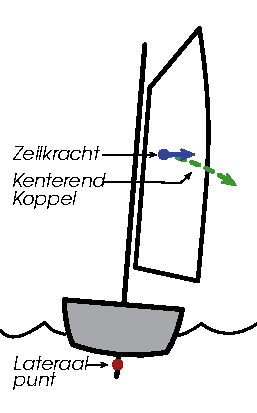
\includegraphics[height=6cm]{Hoofdstukken/Krachten/pdf/stabiliteit_kenternd.pdf}
		\caption{Kenterend koppel}
		\label{pic:kenterende_koppel}
	\end{minipage}
	\hfill
	\begin{minipage}[b]{0.33\textwidth}
		\centering
		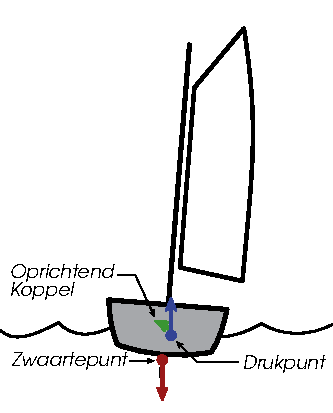
\includegraphics[height=6cm]{Hoofdstukken/Krachten/pdf/stabiliteit_gewichtstabiel.pdf}
		\caption{Oprichtend koppel}
		\label{pic:oprichtend}
	\end{minipage}
	\hfill
	\begin{minipage}[b]{0.32\textwidth}
		\centering
		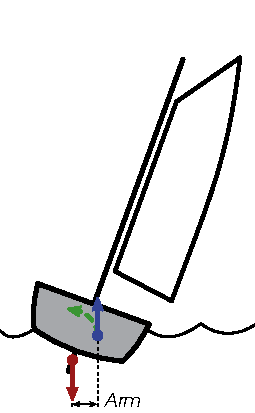
\includegraphics[height=6cm]{Hoofdstukken/Krachten/pdf/stabiliteit_gewichtstabiel_helling.pdf}
		\caption{Helling}
		\label{pic:oprichtend_helling}
	\end{minipage}
\end{figure}

De boot in figuur \ref{pic:vormstabiel} is een vormstabiele boot. Deze wordt gekenmerkt door een hoog zwaartepunt. Dit type schepen heeft een hoge stabiliteit bij een kleine helling. Naarmate de helling toeneemt, zoals in figuur \ref{pic:vormstabiel_helling}, komt het drukpunt dichter naar het zwaartepunt toe. Dit verkleint de arm en hierdoor neemt het oprichtend koppel af en dus ook de stabiliteit.
\begin{figure}[H]
	\centering
	\begin{minipage}[b]{0.49\textwidth}
		\centering
		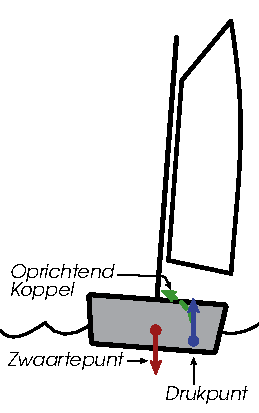
\includegraphics[height=6cm]{Hoofdstukken/Krachten/pdf/stabiliteit_vormstabiel.pdf}
		\caption{Vormstabiel}
		\label{pic:vormstabiel}
	\end{minipage}
	\hfill
	\begin{minipage}[b]{0.49\textwidth}
		\centering
		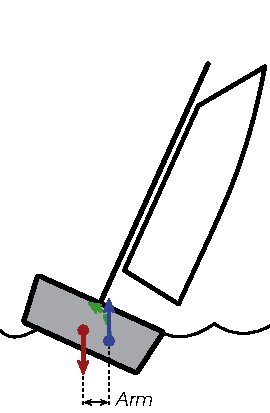
\includegraphics[height=6cm]{Hoofdstukken/Krachten/pdf/stabiliteit_vormstabiel_helling.pdf}
		\caption{Vormstabiel onder helling}
		\label{pic:vormstabiel_helling}
	\end{minipage}
\end{figure}

Stabiliteit van schepen wordt dus gedicteerd door de ligging van het zwaartepunt ten opzichte van het drukpunt. Gewichtsstabiele schepen hebben daarom en lage beginstabiliteit en een hoge eindstabiliteit. Voor vormstabiele schepen is dit andersom. Deze hebben een hoge beginstabiliteit en een lage eindstabiliteit.  

\newpage
\section{Schijnbare wind}
De wind die op een boot werkt bestaat in feiten uit twee delen: de ware wind en de vaartwind.

\begin{enumerate}
	\item De \textbf{ware wind} ontstaat door drukverschillen in de atmosfeer en voel je als je stil staat. De ware wind is ook af te zien aan vlaggen. 
	\item De \textbf{vaartwind} ontstaat daarentegen door de voorwaartse snelheid van het schip. Dit fenomeen is ook te voelen als je op een windstille dag fiets: door de voortbeweging voel je toch wind. 
\end{enumerate}

De ware wind en de vaartwind vormen samen de schijnbare wind. Dit is de wind waar het schip op vooruit gaat en de wind die je in de boot voelt. In figuur \ref{pic:schijnbare_wind} is de schijnbare wind te zien en hoe deze ontstaat vanuit zijn twee componenten. 

\begin{figure}[H]
	\centering
	\begin{minipage}[b]{0.49\textwidth}
		\centering
		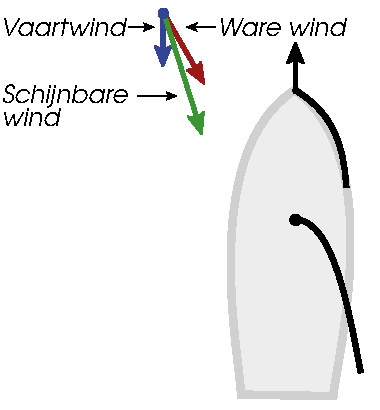
\includegraphics[height=6cm]{Hoofdstukken/Krachten/pdf/wind_schijnbaar.pdf}
		\caption{Schijnbare wind}
		\label{pic:schijnbare_wind}
	\end{minipage}
	\hfill
	\begin{minipage}[b]{0.49\textwidth}
		\centering
		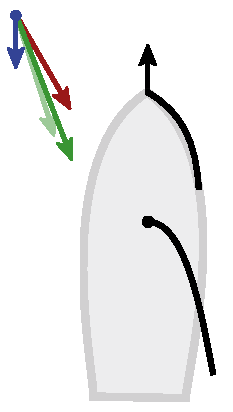
\includegraphics[height=6cm]{Hoofdstukken/Krachten/pdf/wind_vlaag.pdf}
		\caption{Windvlaag}
		\label{pic:windvlaag}
	\end{minipage}
\end{figure}

De samenwerking van de ware wind en de vaartwind geeft een bijzondere dynamiek aan de schijnbare wind. Wanneer de ware wind plots krachtiger wordt, bijvoorbeeld door een windvlaag, zal de wind wat `ruimer' de boot in komen. Dit is te zien in figuur \ref{pic:windvlaag}. Doordat de wind wat ruimer is, is het mogelijk wat hoger te varen. Zo is het mogelijk om tijdens een windvlaag wat hoogte te winnen.

Een tweede effect is dat wanneer de snelheid van het schip toeneemt, en dus ook de vaartwind, de wind juist scherper de boot in komt. Snel varende schepen kunnen daarom wat minder hoog aan de wind varen.

\section{Conclusie}
In dit hoofdstuk zijn de verschillende krachten op het schip behandeld. Je snapt nu onder andere hoe een schip aan zijn voortstuwing komt, wat het effect van het grootzeil en de fok is en wat de invloed van de helling op de boot is. Met deze kennis het is mogelijk meer controle over de boot te krijgen.  